\documentclass{beamer}
\usepackage[utf8]{inputenc}

\usetheme{Madrid}
\usecolortheme{default}
\usepackage{amsmath,amssymb,amsfonts,amsthm}
\usepackage{txfonts}
\usepackage{tkz-euclide}
\usepackage{listings}
\usepackage{adjustbox}
\usepackage{array}
\usepackage{tabularx}
\usepackage{gvv}
\usepackage{lmodern}
\usepackage{circuitikz}
\usepackage{tikz}
\usepackage{graphicx}

\setbeamertemplate{page number in head/foot}[totalframenumber]

\usepackage{tcolorbox}
\tcbuselibrary{minted,breakable,xparse,skins}



\definecolor{bg}{gray}{0.95}
\DeclareTCBListing{mintedbox}{O{}m!O{}}{%
  breakable=true,
  listing engine=minted,
  listing only,
  minted language=#2,
  minted style=default,
  minted options={%
    linenos,
    gobble=0,
    breaklines=true,
    breakafter=,,
    fontsize=\small,
    numbersep=8pt,
    #1},
  boxsep=0pt,
  left skip=0pt,
  right skip=0pt,
  left=25pt,
  right=0pt,
  top=3pt,
  bottom=3pt,
  arc=5pt,
  leftrule=0pt,
  rightrule=0pt,
  bottomrule=2pt,
  toprule=2pt,
  colback=bg,
  colframe=orange!70,
  enhanced,
  overlay={%
    \begin{tcbclipinterior}
    \fill[orange!20!white] (frame.south west) rectangle ([xshift=20pt]frame.north west);
    \end{tcbclipinterior}},
  #3,
}
\lstset{
    language=C,
    basicstyle=\ttfamily\small,
    keywordstyle=\color{blue},
    stringstyle=\color{orange},
    commentstyle=\color{green!60!black},
    numbers=left,
    numberstyle=\tiny\color{gray},
    breaklines=true,
    showstringspaces=false,
}


\title 
{2.2.13}
\date{August 31,2025}


\author 
{Abhiram Reddy-AI25BTECH11021}



\begin{document}


\frame{\titlepage}
\begin{frame}{Question}
The angles between
two vectors a and b with magnitude
$\sqrt{3}$ and 4, respectively,
and a, b= 2 $\sqrt{3}$ is

\end{frame}



\begin{frame}{Given}
\begin{itemize}
    \item \( |\vec{a}| = \sqrt{3} \)
    \item \( |\vec{b}| = 4 \)
    \item \( \vec{a} \cdot \vec{b} = 2\sqrt{3} \)
\end{itemize}
Find the angle \( \theta \) between \( \vec{a} \) and \( \vec{b} \).
\end{frame}

%-----------------------------------
\begin{frame}{Formula for Angle Between Vectors}
\[
\vec{a} \cdot \vec{b} = |\vec{a}| |\vec{b}| \cos\theta
\]
Substitute the given values:
\[
2\sqrt{3} = \sqrt{3} \cdot 4 \cdot \cos\theta
\]
\[
2\sqrt{3} = 4\sqrt{3} \cos\theta
\]
\[
\cos\theta = \frac{2\sqrt{3}}{4\sqrt{3}} = \frac{1}{2}
\]
\[
\theta = \cos^{-1}\left( \frac{1}{2} \right)
\]
\[
\boxed{ \theta = 60^\circ }
\]
\end{frame}



\begin{frame}[fragile]
    \frametitle{C Code }

    \begin{lstlisting}

#include <stdio.h>
#include <math.h>

int main() {
    double dot_product = 2 * sqrt(3);
    double magnitude_a = sqrt(3);
    double magnitude_b = 4.0;

    double cos_theta = dot_product / (magnitude_a * magnitude_b);
    double theta_rad = acos(cos_theta);  // angle in radians
    double theta_deg = theta_rad * (180.0 / M_PI);  // convert to degrees

    printf("cos(theta) = %.6f\n", cos_theta);
    printf("Angle (in radians) = %.6f\n", theta_rad);
    printf("Angle (in degrees) = %.6f\n", theta_deg);

    return 0;
}


    \end{lstlisting}
\end{frame}

\begin{frame}[fragile]
    \frametitle{Python Code}
    \begin{lstlisting}
import matplotlib.pyplot as plt
import numpy as np

# Given values
a_mag = np.sqrt(3)
b_mag = 4
dot_product = 2 * np.sqrt(3)

# Compute angle
cos_theta = dot_product / (a_mag * b_mag)
theta = np.arccos(cos_theta)

# Vector a: along x-axis
a = np.array([a_mag, 0])

# Vector b: rotated by angle theta
b = np.array([b_mag * np.cos(theta), b_mag * np.sin(theta)])

    \end{lstlisting}
\end{frame}

\begin{frame}[fragile]
    \frametitle{Python Code}
    \begin{lstlisting}

# Plot
origin = np.array([0, 0])
plt.quiver(*origin, *a, angles='xy', scale_units='xy', scale=1, color='red', label=r'$\vec{a}$')
plt.quiver(*origin, *b, angles='xy', scale_units='xy', scale=1, color='blue', label=r'$\vec{b}$')

# Annotate the angle
angle_deg = np.degrees(theta)
plt.text(0.5, 0.5, f'$\\theta$ = {angle_deg:.1f}°', fontsize=12)
    \end{lstlisting}
\end{frame}

\begin{frame}[fragile]
    \frametitle{Python Code}
    \begin{lstlisting}

# Plot settings
plt.xlim(0, 5)
plt.ylim(0, 3)
plt.gca().set_aspect('equal')
plt.grid(True)
plt.xlabel("x")
plt.ylabel("y")
plt.title("Angle Between Vectors")
plt.legend()

# Save the plot
plt.savefig("python_plot.png")
plt.show()

    \end{lstlisting}
\end{frame}



\begin{frame}{Plot}
    \centering
    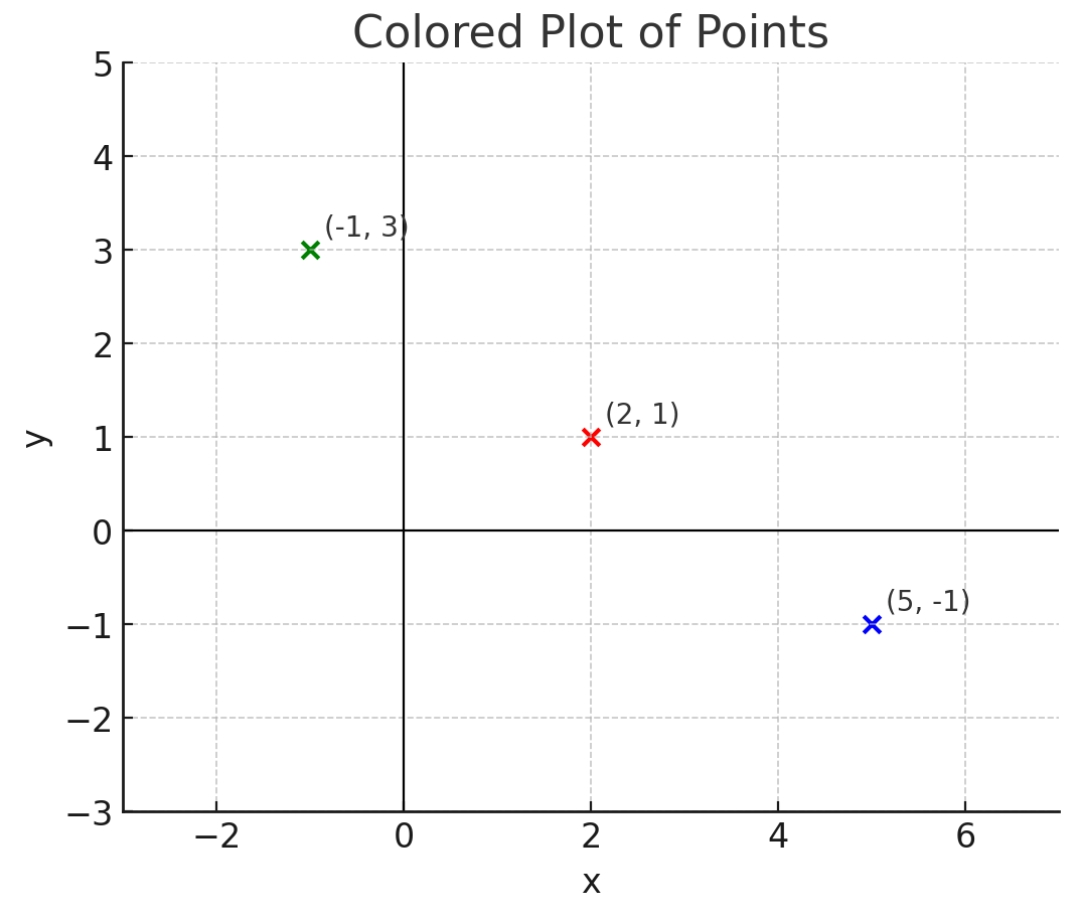
\includegraphics[width=\columnwidth, height=0.8\textheight, keepaspectratio]{figs/python_plot.png}     
\end{frame}


\end{document}